\begin{table}[H]
    \centering
    \begin{tabular}{ccc}
        % \hline
        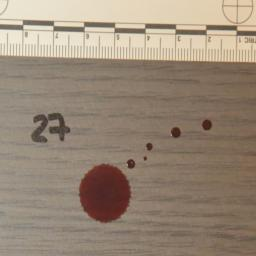
\includegraphics[width=0.20\linewidth]{../asset/data_labo/1_bois_350.jpg} & 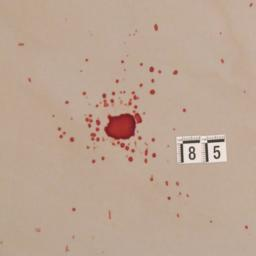
\includegraphics[width=0.20\linewidth]{../asset/data_labo/2_carrelage_523.jpg}& 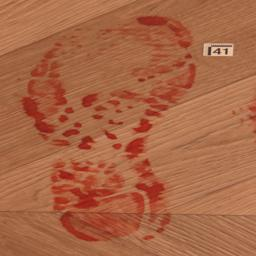
\includegraphics[width=0.20\linewidth]{../asset/data_labo/3_lino_888.jpg} \\
        1- Traces passives & 2- Goutte à Goutte & 3- Transfert par contact \\
        % \hline
        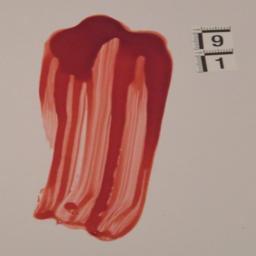
\includegraphics[width=0.20\linewidth]{../asset/data_labo/4_papier_1586.jpg} & 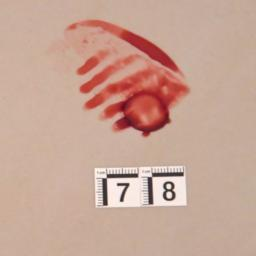
\includegraphics[width=0.20\linewidth]{../asset/data_labo/5_carrelage_5605.jpg} & 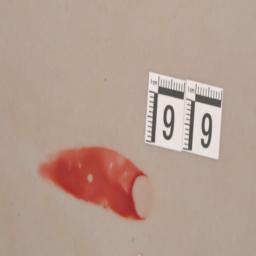
\includegraphics[width=0.20\linewidth]{../asset/data_labo/6_bois_604.jpg} \\
        4- Transfert glissé & 5- Altération par contact & 6- Altération glissée \\
        % \hline
        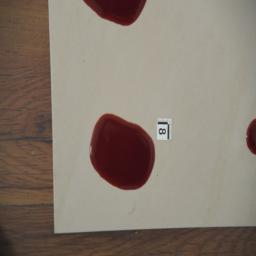
\includegraphics[width=0.20\linewidth]{../asset/data_labo/7_carrelage_5507.jpg} & \includegraphics[width=0.20\linewidth]{../asset/data_labo/8_coulée_4526.jpg} & 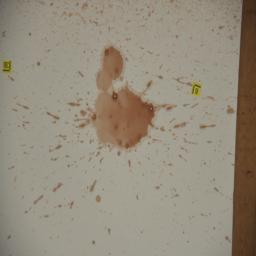
\includegraphics[width=0.20\linewidth]{../asset/data_labo/9_papier_6375.jpg} \\
        7- Accumulation & 8- Coulée & 9- Chute de volume \\
        % \hline
        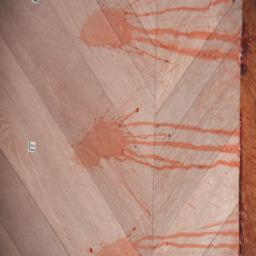
\includegraphics[width=0.20\linewidth]{../asset/data_labo/10_lino_933.jpg} & 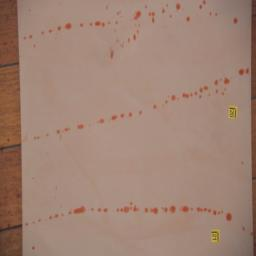
\includegraphics[width=0.20\linewidth]{../asset/data_labo/11_carrelage_905.jpg} & 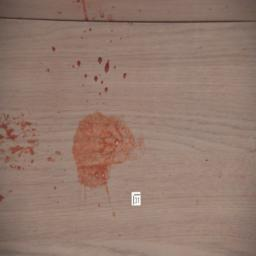
\includegraphics[width=0.20\linewidth]{../asset/data_labo/12_bois_326.jpg} \\
        10- Sang Propulsé & 11- éjection & 12- Volume impacté \\
        % \hline
        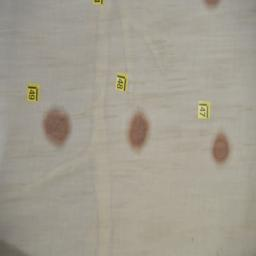
\includegraphics[width=0.20\linewidth]{../asset/data_labo/13_carrelage_7374.jpg} & 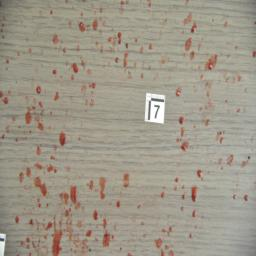
\includegraphics[width=0.20\linewidth]{../asset/data_labo/14_lino_6320.jpg} & 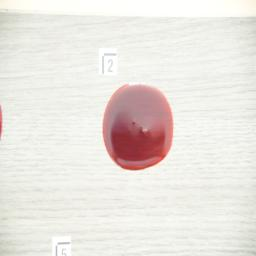
\includegraphics[width=0.20\linewidth]{../asset/data_labo/15_p1040.jpg} \\
        13- Imprégnation & 14- Zone d'interruption & 15- Modèle d'impact \\
        % \hline
        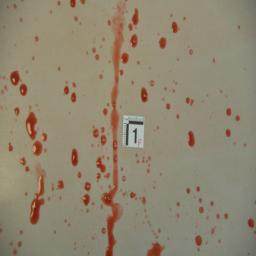
\includegraphics[width=0.20\linewidth]{../asset/data_labo/16_carrelage_598.jpg} & 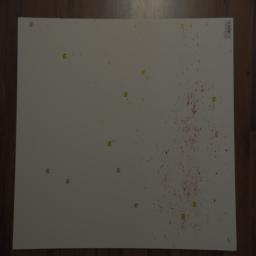
\includegraphics[width=0.20\linewidth]{../asset/data_labo/17_papier_8323.jpg} & 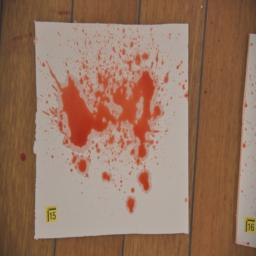
\includegraphics[width=0.20\linewidth]{../asset/data_labo/18_bois_4727.jpg}\\
        16- Foyer de modèle d'impact & 17- Trace gravitationnelle & 18- Sang expiré \\
        % \hline
    \end{tabular}
    \caption{Classe des données de laboratoire et leur exemple en image}
    \label{tab: images of all classes}
\end{table}